\documentclass[11pt]{article}
\usepackage[T1]{fontenc}
\usepackage{amsmath,amssymb}
\usepackage{booktabs}
\usepackage{graphicx}
\usepackage{longtable}
\usepackage{microtype}
\usepackage{xurl}
\usepackage[colorlinks=true,allcolors=blue]{hyperref}
\usepackage[margin=0.85in]{geometry}

\title{Technical Report: Periodic-1D Rank-One Single-Band Fourier Locality}
\author{Project Koios}
\date{Provisional non-retained development calculation, 29 October 2026}

\begin{document}
\maketitle

\section{Scientific question and evidence boundary}

For the lowest ordered eigenvalue field of the exact controlled four-state periodic
parent, how do finite interpolation, deliberate Fourier-support truncation, and direct
Hermitian scalar fitting behave as the construction mesh and retained hopping range are
increased?

This report records a local, non-retained development calculation using the frozen
finite controls.  The calculation result was reconstructed by the independent verifier,
all 725 named verification comparisons passed, and the authenticated two-figure
renderer completed in memory.  No execution directory, sealed evidence package,
release, publication artifact, continuum result, uncertainty estimate, or material
validation was created.  The numerical statements below are therefore provisional
finite-representation results rather than promoted project evidence.

\section{Rank-one structural boundary}

Let $H(q)\in\mathbb{C}$ be the scalar represented Hamiltonian and let
$U(q)\in U(1)$.  Scalar multiplication commutes, so
\begin{equation}
 U(q)^\dagger H(q)U(q)=H(q)U(q)^\dagger U(q)=H(q).
\end{equation}
An internal scalar phase therefore cannot redistribute the represented Hamiltonian
among Fourier hopping coefficients.  This calculation tests scalar interpolation,
truncation, and fit behavior.  It does not test the gauge-dependent represented-operator
locality possible at rank two and above.

\section{Exact parent and finite controls}

The typed parent identity is
\texttt{ksdft2effmass.periodic1d.controlled-four-state-parent.v1}.  It is bound in the
configuration wire to
\begin{equation}
 H(q)=\lambda_0(K(q)),\qquad
 K(q)=T_0+e^{2\pi iq}T_{+1}+e^{-2\pi iq}T_{+1}^{\dagger},
\end{equation}
with
\begin{equation}
T_0=\begin{pmatrix}
-6/5&3/50&0&0\\3/50&-7/20&0&0\\
0&0&1&1/25\\0&0&1/25&7/4
\end{pmatrix},\qquad
T_{+1}=\begin{pmatrix}
3/20&0&3/25&0\\0&-1/10&0&1/10\\
0&0&1/20&0\\0&0&0&-1/25
\end{pmatrix}.
\end{equation}
The entries are exact rational multiples of $E_{\mathrm{ref}}=1$.  Construction sizes
are $N\in\{32,64,128,256\}$, with $N=256$ designated production.  The evaluation
inventory contains 1025 points
\begin{equation}
 q_i=-\frac12+\frac{i+1/257}{1025},\qquad i=0,\ldots,1024,
\end{equation}
constructed as exact rationals before conversion to binary64.  Retained ordinary
supports are $R=0,\ldots,15$.  The sampled-gap threshold is
$0.25E_{\mathrm{ref}}$, the application error threshold is
$10^{-8}E_{\mathrm{ref}}$, and the final adjacent-mesh refinement tolerance is
$10^{-10}$ on the declared channel vector.

For each construction mesh, the complete cyclic interpolant $I_N$, transform-mediated
truncation $T_{N,R}$, and direct Hermitian scalar fit $D_{N,R}$ are compared on the
disjoint evaluation inventory.  The reported channels include
\begin{align}
 e_{\mathrm{int}}(N)&=\max_q |H(q)-I_N(q)|,\\
 e_{\mathrm{trunc}}(N,R)&=\max_q |I_N(q)-T_{N,R}(q)|,\\
 e_{\mathrm{med}}(N,R)&=\max_q |H(q)-T_{N,R}(q)|,\\
 e_{\mathrm{dir}}(N,R)&=\max_q |H(q)-D_{N,R}(q)|.
\end{align}
The producer calculates the result once.  Independent verification reconstructs the
parent eigensystems, Fourier sums, direct least-squares systems, diagnostics, masks,
threshold decisions, refinement inventory, sampled-gap minimizer, and visualization
projection without invoking the production analyzer.

\section{Finite numerical results}

\subsection{Sampled gap and qualification disposition}

The minimum sampled first-to-second parent eigenvalue gap was
\begin{equation}
 \Delta_{\min}=0.37249453282422684\,E_{\mathrm{ref}}.
\end{equation}
It occurred on the production construction mesh at index 128, $q=0$.  The value exceeds
the declared sampled threshold $0.25E_{\mathrm{ref}}$.  This is a qualification over the
finite sampled inventories only; it is not a global isolation certificate.

The first range at which both transform-mediated and direct-fit total maximum errors
were at or below $10^{-8}E_{\mathrm{ref}}$ was $R=11$ for every construction mesh.
Passage remained sustained through $R=15$.  The maximum final $N=128$ to $N=256$
channel change was $6.2211547825082476\times10^{-15}$, below the declared
$10^{-10}$ tolerance.  The resulting bounded finite qualification disposition was
\emph{pass}.  That disposition does not imply continuum convergence or scientific
validation.

\subsection{Mesh-dependent interpolation and representation diagnostics}

\begin{table}[htbp]
\centering
\caption{Finite construction-mesh diagnostics in units of $E_{\mathrm{ref}}$.}
\begin{tabular}{rrrrrr}
\toprule
$N$ & reconstruction max. & Hermiticity max. & interpolation max. & interpolation RMS & first pass \\
\midrule
32  & $4.441\times10^{-16}$ & $1.310\times10^{-18}$ & $2.234057\times10^{-11}$ & $1.077042\times10^{-11}$ & 11 \\
64  & $4.449\times10^{-16}$ & $9.136\times10^{-18}$ & $8.882\times10^{-16}$ & $2.903\times10^{-16}$ & 11 \\
128 & $4.458\times10^{-16}$ & $1.676\times10^{-17}$ & $1.110\times10^{-15}$ & $3.052\times10^{-16}$ & 11 \\
256 & $6.670\times10^{-16}$ & $2.815\times10^{-17}$ & $8.882\times10^{-16}$ & $3.121\times10^{-16}$ & 11 \\
\bottomrule
\end{tabular}
\end{table}

The interpolation maximum fell from $2.234057\times10^{-11}$ at $N=32$ to values near
binary64 roundoff for $N\ge64$.  The adjacent-mesh maximum channel changes for
$32\rightarrow64$, $64\rightarrow128$, and $128\rightarrow256$ were respectively
$2.2339685656902475\times10^{-11}$, $4.17817502814292\times10^{-15}$, and
$6.2211547825082476\times10^{-15}$.  These are finite adjacent-mesh diagnostics, not a
continuum error estimate.

Every attained production support was nondominated under the declared
$(R,e_{\mathrm{med}})$ ordering because the mediated total maximum error decreased
strictly over $R=0,\ldots,15$.  No production supports formed a near-tie under the
mixed $10^{-12}$ comparison rule.

\subsection{Production support and error table}

\begingroup
\small
\setlength{\tabcolsep}{4pt}
\begin{longtable}{r@{\quad}rrrrr}
\caption{Production $N=256$ range diagnostics in units of $E_{\mathrm{ref}}$.  Displayed values are rounded; typed result bytes retain binary64 values.}\\
\toprule
$R$ & $e_{\mathrm{trunc}}$ & $e_{\mathrm{med}}$ & $e_{\mathrm{dir}}$ & omitted $L^2$ & coefficient defect $L^2$ \\
\midrule
\endfirsthead
\toprule
$R$ & $e_{\mathrm{trunc}}$ & $e_{\mathrm{med}}$ & $e_{\mathrm{dir}}$ & omitted $L^2$ & coefficient defect $L^2$ \\
\midrule
\endhead
0  & $2.969490\times10^{-1}$ & $2.969490\times10^{-1}$ & $2.969490\times10^{-1}$ & $2.094025\times10^{-1}$ & $4.441\times10^{-16}$ \\
1  & $1.529255\times10^{-3}$ & $1.529255\times10^{-3}$ & $1.529255\times10^{-3}$ & $7.868300\times10^{-4}$ & $4.455\times10^{-16}$ \\
2  & $4.702662\times10^{-4}$ & $4.702662\times10^{-4}$ & $4.702662\times10^{-4}$ & $2.415628\times10^{-4}$ & $4.462\times10^{-16}$ \\
3  & $1.454887\times10^{-4}$ & $1.454887\times10^{-4}$ & $1.454887\times10^{-4}$ & $7.488650\times10^{-5}$ & $4.618\times10^{-16}$ \\
4  & $4.475369\times10^{-5}$ & $4.475369\times10^{-5}$ & $4.475369\times10^{-5}$ & $2.309687\times10^{-5}$ & $4.498\times10^{-16}$ \\
5  & $1.366150\times10^{-5}$ & $1.366150\times10^{-5}$ & $1.366150\times10^{-5}$ & $7.070482\times10^{-6}$ & $4.752\times10^{-16}$ \\
6  & $4.136042\times10^{-6}$ & $4.136042\times10^{-6}$ & $4.136042\times10^{-6}$ & $2.146950\times10^{-6}$ & $4.673\times10^{-16}$ \\
7  & $1.241321\times10^{-6}$ & $1.241321\times10^{-6}$ & $1.241321\times10^{-6}$ & $6.463664\times10^{-7}$ & $4.778\times10^{-16}$ \\
8  & $3.691080\times10^{-7}$ & $3.691080\times10^{-7}$ & $3.691080\times10^{-7}$ & $1.928393\times10^{-7}$ & $4.717\times10^{-16}$ \\
9  & $1.086649\times10^{-7}$ & $1.086649\times10^{-7}$ & $1.086649\times10^{-7}$ & $5.697590\times10^{-8}$ & $4.599\times10^{-16}$ \\
10 & $3.164491\times10^{-8}$ & $3.164491\times10^{-8}$ & $3.164491\times10^{-8}$ & $1.665750\times10^{-8}$ & $4.590\times10^{-16}$ \\
11 & $9.105412\times10^{-9}$ & $9.105412\times10^{-9}$ & $9.105413\times10^{-9}$ & $4.813878\times10^{-9}$ & $4.783\times10^{-16}$ \\
12 & $2.584796\times10^{-9}$ & $2.584796\times10^{-9}$ & $2.584796\times10^{-9}$ & $1.373266\times10^{-9}$ & $4.830\times10^{-16}$ \\
13 & $7.224646\times10^{-10}$ & $7.224646\times10^{-10}$ & $7.224648\times10^{-10}$ & $3.860166\times10^{-10}$ & $4.757\times10^{-16}$ \\
14 & $1.982817\times10^{-10}$ & $1.982817\times10^{-10}$ & $1.982825\times10^{-10}$ & $1.066565\times10^{-10}$ & $5.409\times10^{-16}$ \\
15 & $5.322764\times10^{-11}$ & $5.322764\times10^{-11}$ & $5.322831\times10^{-11}$ & $2.886786\times10^{-11}$ & $5.372\times10^{-16}$ \\
\bottomrule
\end{longtable}
\endgroup

At $R=10$, both total maximum errors remained above the application threshold.  At
$R=11$, the mediated and direct values were respectively
$9.105412313026306\times10^{-9}$ and
$9.105412868137819\times10^{-9}$, producing the first joint passage.  The direct and
transform-mediated coefficient vectors agreed to approximately
$4.4\times10^{-16}$--$5.4\times10^{-16}$ in $L^2$ over the production range inventory;
the maximum sampled route defect was $1.5544\times10^{-15}E_{\mathrm{ref}}$.  This
agreement is specific to the finite scalar control and the implemented binary64 routes.

The complete production coefficient magnitudes were symmetric to numerical precision.
The dominant values were $|t_0|=1.2116915623409472E_{\mathrm{ref}}$ and
$|t_{\pm1}|\approx0.1480688936028328E_{\mathrm{ref}}$.  Magnitudes then decreased from
$5.295039809188736\times10^{-4}$ at $|R|=2$ to approximately
$7.26\times10^{-11}$ at $|R|=15$.  The largest production Parseval absolute residual
across the retained ranges was $1.3877787807814457\times10^{-17}E_{\mathrm{ref}}^2$.

\section{Authenticated provisional figures}

Figures~\ref{fig:locality} and~\ref{fig:routes} render only the authenticated projection
from the passing in-memory verification.  They are retained here as provisional report
illustrations, not as an execution package, sealed evidence, or publication figure set.

\begin{figure}[p]
\centering
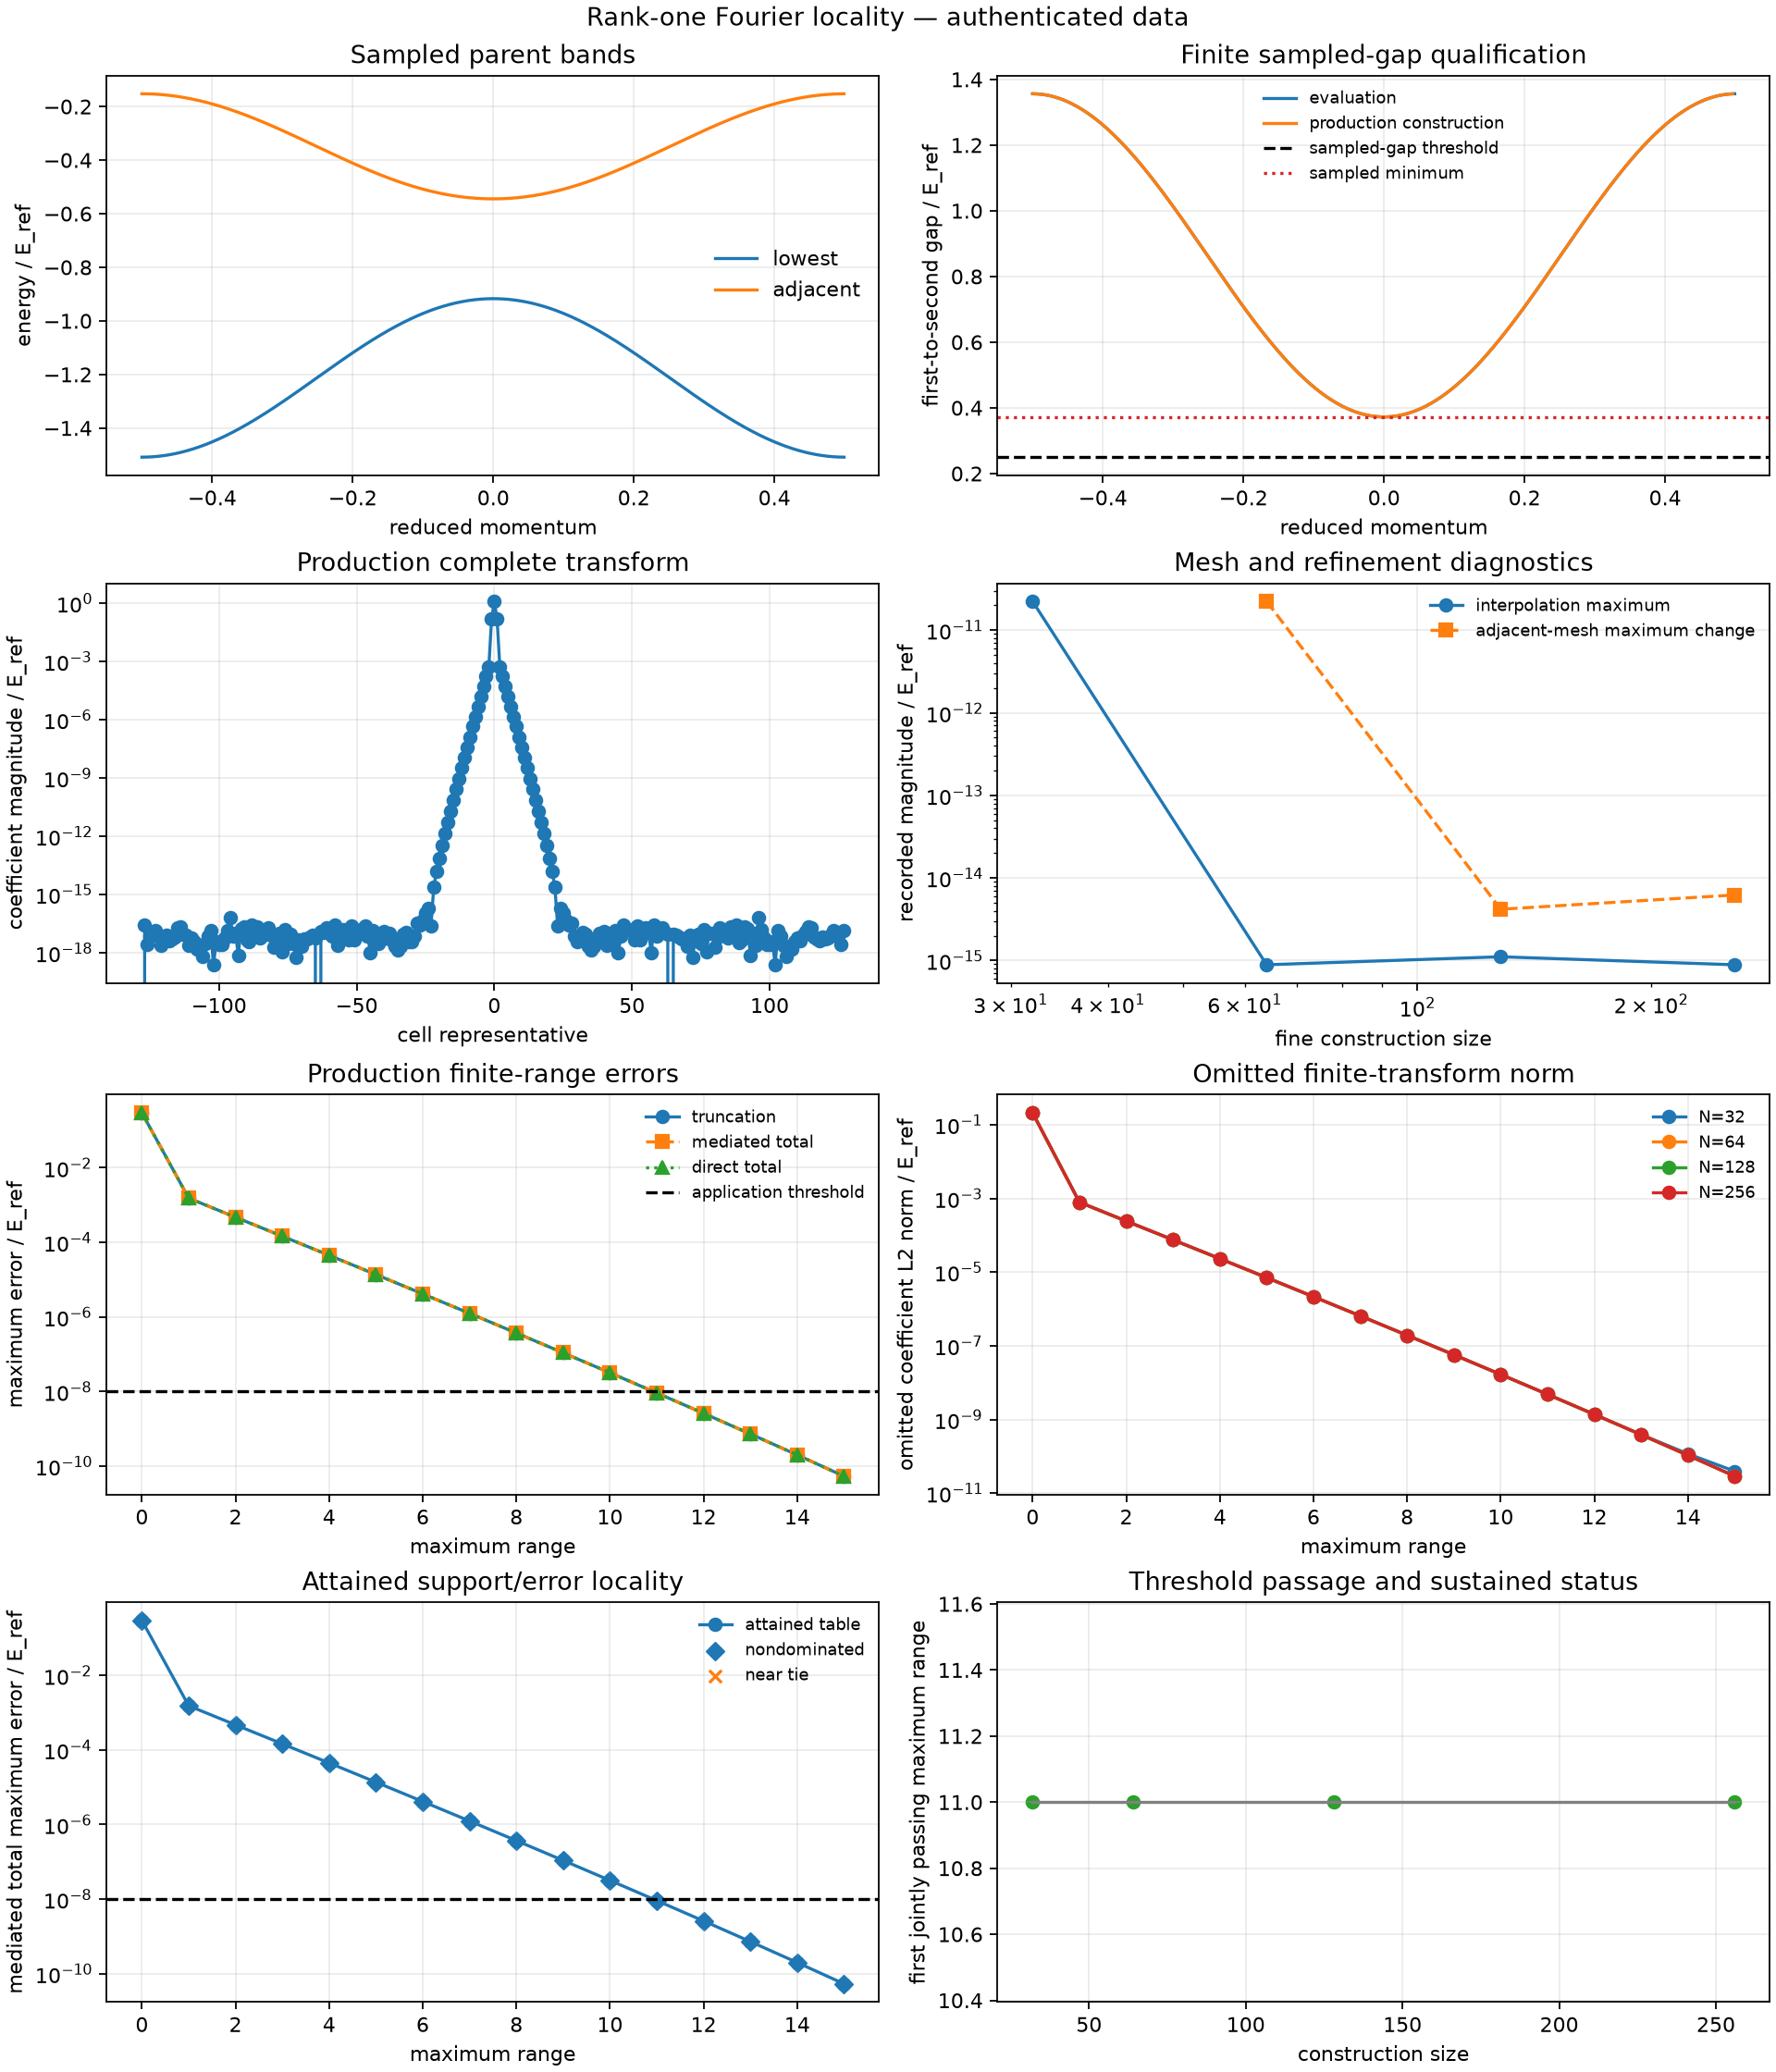
\includegraphics[width=\textwidth,height=0.90\textheight,keepaspectratio]{rank1-fourier-locality.png}
\caption{Authenticated finite rank-one Fourier-locality projection.  The eight panels
show the sampled parent bands; evaluation and production sampled gaps with their finite
threshold; complete production coefficient decay; interpolation and adjacent-mesh
refinement; production truncation, mediated-total, and direct-total errors; omitted
coefficient norms; attained support/error masks; and first sustained threshold passage.
All quantities are finite binary64 diagnostics.}
\label{fig:locality}
\end{figure}

\begin{figure}[p]
\centering
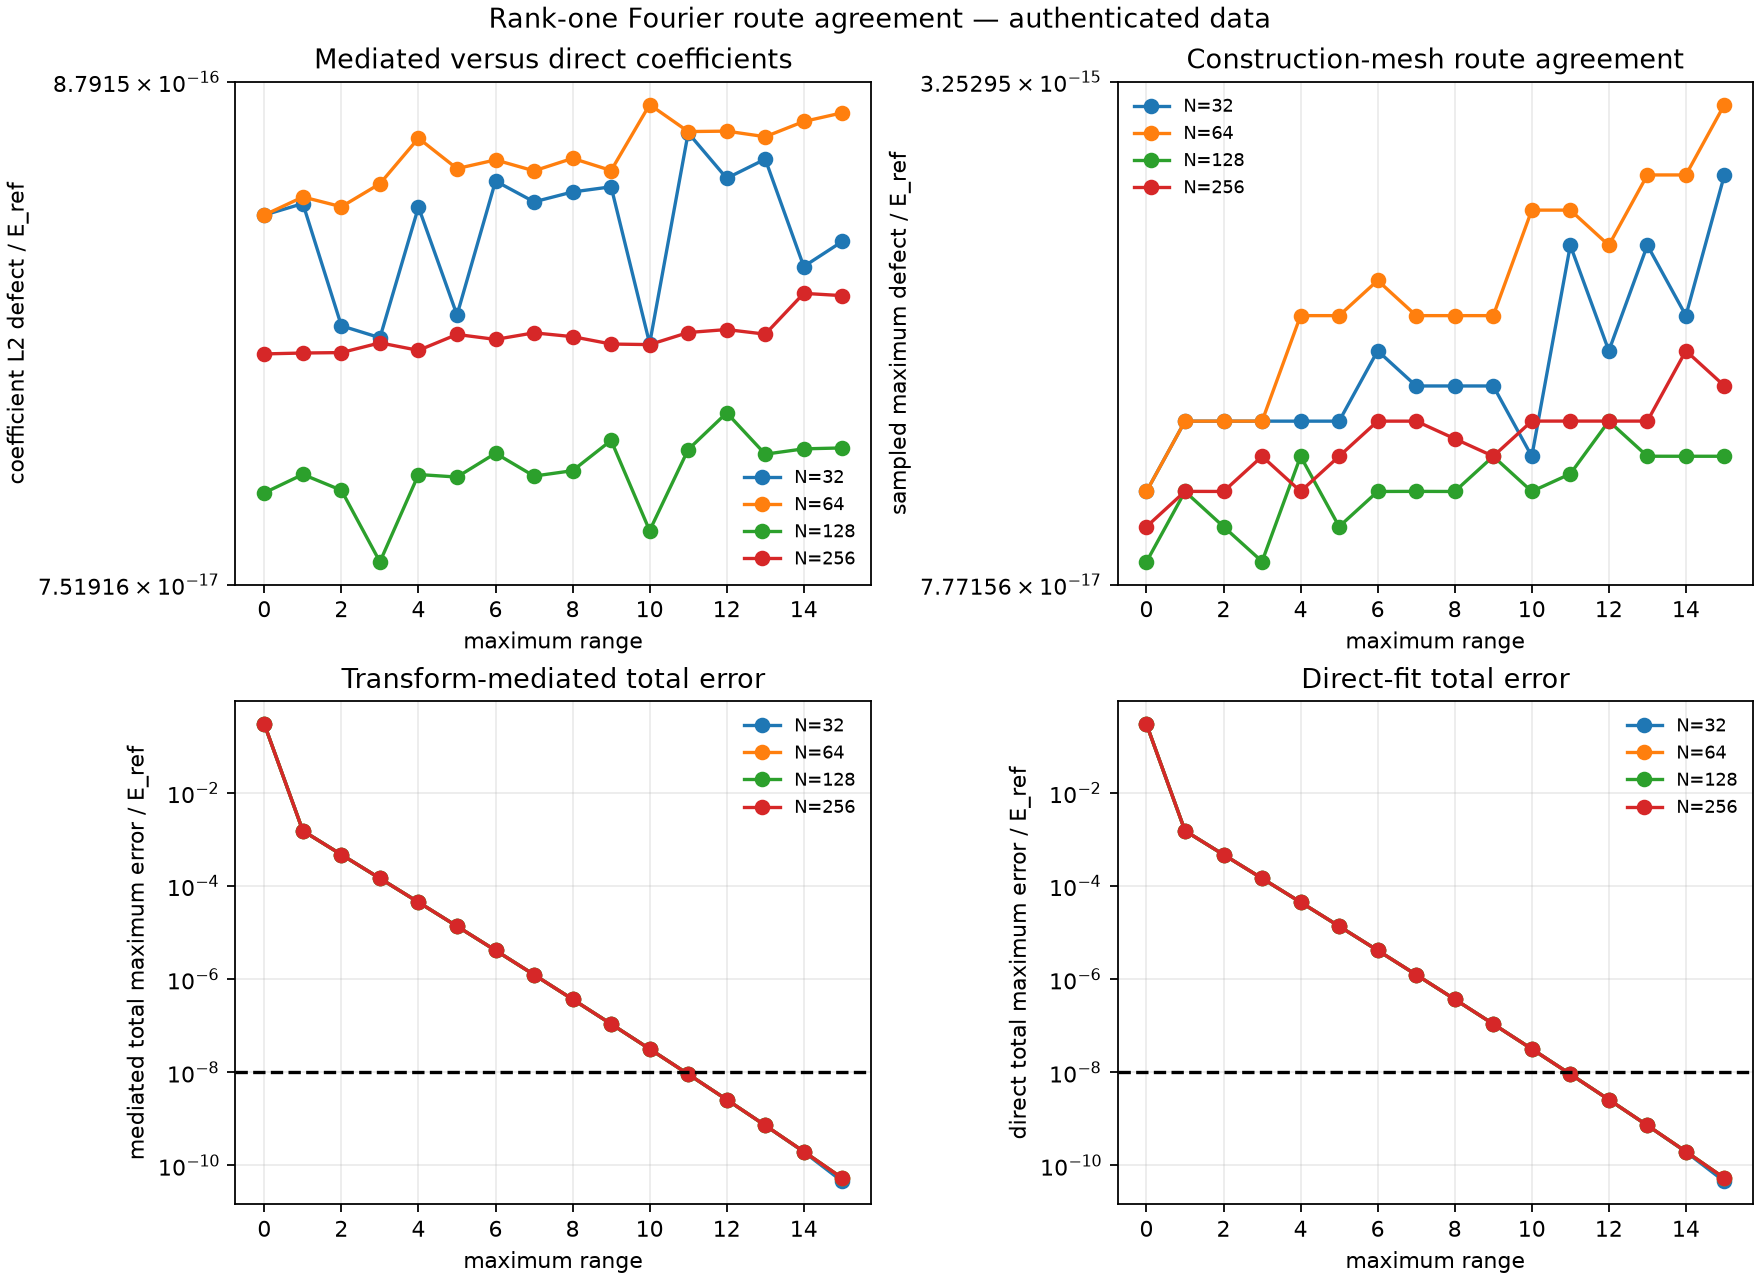
\includegraphics[width=\textwidth,height=0.82\textheight,keepaspectratio]{rank1-fourier-route-agreement.png}
\caption{Authenticated finite route-agreement projection.  The upper panels show the
coefficient-vector and construction-sample defects between transform-mediated and direct
Hermitian fits.  The lower panels show the two total-error routes and the declared
$10^{-8}E_{\mathrm{ref}}$ application threshold.}
\label{fig:routes}
\end{figure}
\clearpage

\section{Independent verification and authenticated presentation}

The byte-owning verifier reconstructed the typed result from the same immutable bytes
used for its subject SHA-256.  It independently regenerated the exact evaluation
coordinates, bound parent identity, parent spectra, complete Fourier coefficients,
truncated and direct candidates, error and norm diagnostics, design ranks and condition
numbers, Pareto and near-tie masks, first and sustained passage, max/RMS triangle checks,
refinement labels and values, sampled-gap minimizer and threshold side, finite
qualification disposition, and every field of the visualization projection.

All 725 named observations passed.  The largest observed discrepancy was
$9.672262990534364\times10^{-12}$; its comparison remained within the applicable mixed
tolerance, and the largest tolerance in the aggregate was
$1.2691051231735601\times10^{-11}$.  A passing software/numerical aggregate verifies the
declared finite operations and correlations only.  It does not establish a Formal
certificate or scientific validation.

The authenticated renderer produced the two PNG values embedded in
Figures~\ref{fig:locality} and~\ref{fig:routes}.  Their exact bytes are retained only as
technical-report review illustrations.  They were not copied into a retained execution,
sealed evidence package, or publication asset inventory.

\section{Provisional provenance}

The development calculation used branch
\nolinkurl{work/periodic1d-rank1-control-v3} at base revision
\nolinkurl{bc1601f3a50dda19b994eea474ca522f2d836c26} in a dirty worktree.  Runtime on the
local development machine was approximately 1.12 seconds for calculation, 0.19 seconds
for independent verification, and 0.88 seconds for rendering.  Timings are descriptive,
not benchmarks.

Exact SHA-256 identities from this non-retained development calculation were:
\begin{itemize}
\item configuration bytes: \nolinkurl{5c9beb47eefe9749a249a74545a25c7ef8d3dd6eafec658d23dfbee574ace173};
\item result bytes: \nolinkurl{3f24fbf6bd6d85040e98481b0487407932f43a70dd04690417396a50797fad2b};
\item verification bytes: \nolinkurl{69232918f32f7006df0a5818925c35ff1462d4120448692aebdfc4a1489fd366};
\item visualization-data bytes: \nolinkurl{5fd7fb9bf56c18cf112ae1060b672d1990c5cfc97661321eac4c735fdb816f3a};
\item locality report PNG: \nolinkurl{df7032249383521b91012d18ef83025a72e6333b387e6b97b9acc898b2fdff62};
\item route-agreement report PNG: \nolinkurl{c95f9ab1289baefffba637197d40218324f46c9b2b18476a8bccf2067352cf07}.
\end{itemize}
These hashes identify the exact development bytes only.  They do not seal, promote, or
publish them.  No retained result or verification file currently exists in the
repository.

\section{Conclusions and limitations}

Within the declared finite binary64 control, the lowest eigenvalue field has a rapidly
decreasing scalar Fourier tail, construction meshes $N\ge64$ agree on the evaluation
inventory near roundoff, and both retained approximation routes first satisfy the
$10^{-8}E_{\mathrm{ref}}$ application threshold at $R=11$.  The sampled gap and final
adjacent-mesh stability gates pass, and all attained production supports are
nondominated because error decreases strictly with range.

These conclusions are deliberately bounded.  They do not establish a continuum limit,
a global isolated band, uncertainty quantification, higher-rank gauge behavior,
material applicability, publication acceptance, evidence sealing, or a Project
Koios--Formal proposition.  Retention or promotion requires a separately authorized
direct execution and the repository's provenance and sealing gates.

\end{document}
